\section{Filtering}
Filtering of raw point clouds is required because of several different reasons. The number of points delivered to the modelling component from the raw point clouds is huge, so filtering non-interesting points away creating a region-of-interest (ROI) in the raw point clouds. Lowering the number points in each cloud delivered to the modelling component is required such the workload can be kept within an acceptable range. The number of points can be further reduced by down-sampling the points left in the ROI by the cut-off filter. A voxel-grid filter utilised for down-sampling also creates the advantage of equal sampling density, but the disadvantage is that the down-sampling means loss of information, and therefore there is a trade off between speed and level of detail of the reconstruction process.

\subsection{Point cloud library}
The Point Cloud Library (PCL) utilised in this project is a library which provide functionality for working on 3D point clouds. PCL delivers a variety of functionality such as filters, segmentation, surface reconstruction, kd- and oc-trees, visualisation, etc. PCL can be found at http://www.pointclouds.org/, along with documentation and tutorials.

\subsection{Point cloud transformation}
Messages received from the vision layer needs to be processed before filtering. This is because the messages delivered to the modelling component contain a point cloud and a pose of the current camera view. The coordinates of the individual points in the cloud are related to the camera frame, but this frame is moving around the object so a transformation of points is needed such they can be related a common static frame.
\begin{figure}[htb]
	\begin{center}
		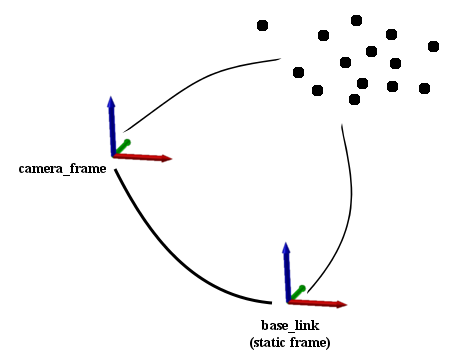
\includegraphics[scale=0.7,trim=0 0 0 0]{graphics/07_modelling/pctransform.png}%trim=l b r t
		\caption{Illustrates points in different frames.}
		\label{fig:filtering_transform}
	\end{center}
\end{figure}

\subsection{Cut-off filter}
The cut-off filter utilised is the implementation from PCL, \texttt{pcl::PassThrough< \ldots >}. A cut-off filter is utilised to create a ROI in the transformed point cloud, partly because the number of points needs to be reduced with respect to processing time and then because the region in which the object resides is fairly small to the region which is recorded by the camera.

\subsection{Voxel-grid filter}
The voxel-grid down-samples the left overs from the cut-off filtering. The down-sampling causes loss of information which mean that surface details are lost in the process, so the amount of down-sampling should be chosen with respect to processing time versus level of detail to be reconstructed. The PCL library luckily have such functionality (\texttt{pcl::VoxelGrid< \ldots >}) which is utilised in the filtering sub-component.\\
\\
The voxel-grid filter works by splitting down the ROI into smaller regions (voxels) of certain resolution in which each of the voxels are analysed. Figure \ref{fig:filtering_voxel_grid} show the principle of the voxel-grid. A new point is approximated for each voxel, the new point is approximated by the points centroid which is contained in the voxel. This method is a little slower compared to just placing the new point in the center of the voxel, but it helps save some more detailed information about the surface curvature.
\begin{figure}[htb]
	\begin{center}
		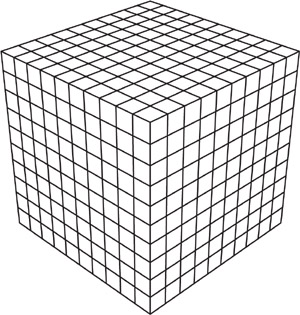
\includegraphics[scale=0.7,trim=0 0 0 0]{graphics/07_modelling/cube.jpg}%trim=l b r t
		\caption{Illustrates a cube consisting of 10x10x10 cubes which resembles the voxel-grid filter.}
		\label{fig:filtering_voxel_grid}
	\end{center}
\end{figure}

\subsection{Point cloud stitching}